\documentclass{standalone}
\usepackage{mathpazo}
\usepackage{siunitx}
\usepackage{amsmath}
\usepackage[american voltages, american currents, american inductors]{circuitikz}
\newcommand*{\equal}{=}

\begin{document}
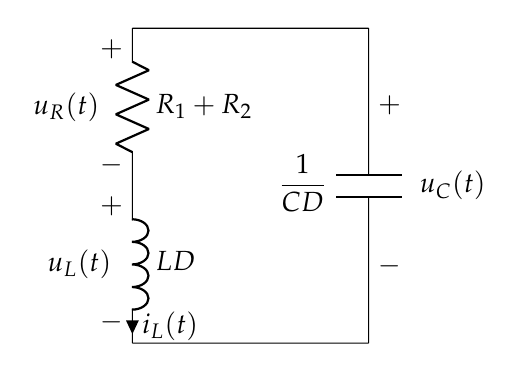
\begin{tikzpicture}
  \coordinate (A) at (0,4);
  \coordinate (B) at (2,4);
  \coordinate (C) at (5,4);
  \coordinate (D) at (0,0);
  \coordinate (E) at (2,0);
  \coordinate (F) at (5,0);
  \draw
  (B) to [R, l = $R_1 + R_2$, v = $u_R(t)$] ++(0, -2)
  to [L, l = $LD$, i = $i_L(t)$, v = $u_L(t)$] (E)
  (C) to [C, l_= $\dfrac{1}{CD}$, v^= $u_C(t)$] (F)
  (E) to [short] (F)
  (B) to [short] (C);
  \end{tikzpicture}
\end{document}